\tikzset{
    ->, 
    level distance = 22em,
    minimum size=2em,
    %edge from parent/.style={draw,thick},
    level 1/.style={sibling distance=6em},
    level 2/.style={sibling distance=3em},
    thick/.style = {line width=1.5pt},
    extra thick/.style = {line width=3.5pt},
    red node/.style={shape=circle,draw=red,fill=red!40,thick,inner sep=1.2},
    blue node/.style={shape=circle,draw=blue,fill=blue!40,thick,inner sep=1.2}
}

\tikzstyle{round}=[thick,draw=black,circle]

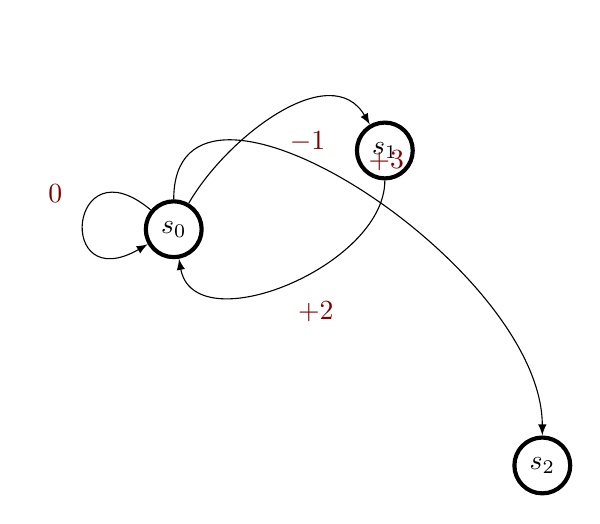
\begin{tikzpicture}[auto,node distance=58mm,>=latex]
    \tikzstyle{round}=[thick,draw=black,circle]
    \node[round] (s0) {$s_0$};
    \node[round, above=10mm, right=23mm] (s1) {$s_1$};
    \node[round, below=30mm, right=43mm] (s2) {$s_2$};

    \draw[->] (s0) [out=60,in=120] to node {} node [swap] {\textcolor{Maroon}{$-1$}} (s1);
    \draw[->] (s1) [out=-90,in=-80] to node {\textcolor{Maroon}{$+2$}} node [swap] {} (s0);
    \draw[->] (s0) [out=90,in=90] to node {\textcolor{Maroon}{$+3$}} node [swap] {} (s2);
    \draw[->] (s0) [out=140,in=210,loop] to node {} node [swap] {\textcolor{Maroon}{$0$}} (s0);




\end{tikzpicture}
